% =====================================================================
%  Standard Sindhi Braille in software
%
%  Compile with XeLaTeX. On Overleaf: Menu -> Compiler -> XeLaTeX.
%  pdfLaTeX will not typeset the Sindhi; see README.md for the fallback.
%
%  Every figure and table of data comes from generated.tex, which is
%  written by make_paper_tables.py out of the same modules the software
%  runs on. Do not edit generated.tex by hand.
% =====================================================================
\documentclass[11pt,a4paper]{article}

\usepackage[margin=2.6cm]{geometry}
\usepackage{fontspec}
\usepackage{booktabs}
\usepackage{longtable}
\usepackage{amsmath}
\usepackage{tikz}
\usepackage{microtype}
\usepackage[hidelinks]{hyperref}
\usepackage{xcolor}
\usepackage{caption}
\usetikzlibrary{positioning, arrows.meta}

% ---- the Sindhi face -------------------------------------------------
% Substitute Scheherazade New or Amiri if Noto Naskh Arabic is unavailable.
\newfontfamily\sdfont{Noto Naskh Arabic}[Script=Arabic]

% ---- a braille cell, drawn from its dot numbers ----------------------
% Every cell in this paper is drawn from the same dot numbers the embosser
% is sent, so a cell printed here cannot disagree with a cell on paper.
\newcommand{\bcell}[1]{%
  \begin{tikzpicture}[baseline=-0.55ex, x=1.75mm, y=1.75mm]
    \foreach \x/\y in {0/2, 0/1, 0/0, 1/2, 1/1, 1/0}
      {\fill[black!17] (\x,\y) circle (0.20);}
    % dot d sits in column (d>3) and row (d-1) mod 3, counting down from the top
    \foreach \d in {#1}{%
      \pgfmathsetmacro{\cx}{\d > 3 ? 1 : 0}%
      \pgfmathsetmacro{\cy}{2 - int(mod(\d - 1, 3))}%
      \fill (\cx,\cy) circle (0.44);}
  \end{tikzpicture}%
}

\newcommand{\pass}{\textcolor{black!70}{\small pass}}
\newcommand{\fail}{\textbf{FAIL}}
\newcommand{\skipped}{\textcolor{black!45}{\small skip}}

\captionsetup{font=small, labelfont=bf}

% ---- figures, generated -------------------------------------------
\newcommand{\NLetters}{52}
\newcommand{\NMeanings}{95}
\newcommand{\NCellsUsed}{59}
\newcommand{\NCellsTotal}{63}
\newcommand{\NShared}{23}
\newcommand{\NThreeWay}{9}
\newcommand{\NChecks}{12}
\newcommand{\NChecksPassed}{11}

\newcommand{\AlphabetTable}{%
% generated by make_paper_tables.py -- do not edit
\begin{LTR}
\begin{longtable}{llll llll}
\toprule
\sd{ا} & \bcell{1} & \sd{ب} & \bcell{1,2} & \sd{ٻ} & \bcell{2,6} & \sd{ڀ} & \bcell{2,3} \\
\sd{ت} & \bcell{2,3,4,5} & \sd{ٿ} & \bcell{1,2,5,6} & \sd{ٽ} & \bcell{2,4,6} & \sd{ٺ} & \bcell{1,3,5} \\
\sd{ث} & \bcell{1,4,5,6} & \sd{پ} & \bcell{1,2,3,4} & \sd{ج} & \bcell{2,4,5} & \sd{ڄ} & \bcell{3,5,6} \\
\sd{ڃ} & \bcell{3,5} & \sd{چ} & \bcell{1,4} & \sd{ڇ} & \bcell{1,6} & \sd{ح} & \bcell{1,5,6} \\
\sd{خ} & \bcell{1,3,4,6} & \sd{د} & \bcell{1,4,5} & \sd{ڌ} & \bcell{1,2,3,6} & \sd{ڏ} & \bcell{3,4} \\
\sd{ڊ} & \bcell{3,4,6} & \sd{ڍ} & \bcell{2,5,6} & \sd{ذ} & \bcell{2,3,4,6} & \sd{ر} & \bcell{1,2,3,5} \\
\sd{ڙ} & \bcell{1,2,4,5,6} & \sd{ز} & \bcell{1,3,5,6} & \sd{س} & \bcell{2,3,4} & \sd{ش} & \bcell{1,4,6} \\
\sd{ص} & \bcell{1,2,3,4,6} & \sd{ض} & \bcell{1,2,4,6} & \sd{ط} & \bcell{2,3,4,5,6} & \sd{ظ} & \bcell{1,2,3,4,5,6} \\
\sd{ع} & \bcell{1,2,3,5,6} & \sd{غ} & \bcell{1,2,6} & \sd{ف} & \bcell{1,2,4} & \sd{ڦ} & \bcell{2,3,5} \\
\sd{ق} & \bcell{1,2,3,4,5} & \sd{ڪ} & \bcell{1,3} & \sd{ک} & \bcell{1,3} \bcell{2,3,6} & \sd{گ} & \bcell{1,2,4,5} \\
\sd{ڳ} & \bcell{1,3,4,5,6} & \sd{ڱ} & \bcell{2,3,5,6} & \sd{ل} & \bcell{1,2,3} & \sd{م} & \bcell{1,3,4} \\
\sd{ن} & \bcell{1,3,4,5} & \sd{ڻ} & \bcell{3,4,5,6} & \sd{و} & \bcell{2,4,5,6} & \sd{ه} & \bcell{1,2,5} \\
\sd{ھ} & \bcell{2,3,6} & \sd{ي} & \bcell{2,4} & \sd{ء} & \bcell{3} & \sd{آ} & \bcell{3,4,5} \\
\bottomrule
\end{longtable}
\end{LTR}
}

\newcommand{\AmbiguityTable}{%
% generated by make_paper_tables.py -- do not edit
\begin{LTR}\footnotesize
\begin{longtable}{clp{0.31\linewidth}p{0.34\linewidth}}
\caption{Every cell the code assigns more than one reading, with the criterion that resolves it. Generated from the implemented tables.}\label{tab:ambiguity}\\
\toprule
cell & dots & readings & resolved by \\
\midrule\endhead
\bcell{2} & \texttt{2} & zabar (diacritic); comma (punctuation); 1 (lower digit); decimal point (sign); pen-name mark (sign) & diacritic after a letter · comma after a completed word · decimal point inside a number · lower 1 after a number sign · and immediately before a pen-name in verse \\[2pt]
\bcell{2,5} & \texttt{25} & jazam (diacritic); colon (punctuation); 3 (lower digit); ratio mark (sign) & colon or jazam in prose · ratio when a fresh number sign follows · lower 3 after a number sign \\[2pt]
\bcell{3,5} & \texttt{35} & \sd{ڃ} (letter); double zer (diacritic); 9 (lower digit); footnote mark (sign) & letter · diacritic after a letter · lower digit after a number sign · the same cell twice is a footnote \\[2pt]
\bcell{3} & \texttt{3} & \sd{ء} (letter); doubling mark (sign); blank line (sign) & the letter \sd{ء} inside a word · the same cell twice after a word means the word is repeated · three of them is a blank line \\[2pt]
\bcell{2,3} & \texttt{23} & \sd{ڀ} (letter); semicolon (punctuation); 2 (lower digit) & letter inside a word · semicolon at the end · lower digit after a number sign \\[2pt]
\bcell{2,6} & \texttt{26} & \sd{ٻ} (letter); double pesh (diacritic); 5 (lower digit) & letter · diacritic after a letter · lower digit after a number sign \\[2pt]
\bcell{2,3,5} & \texttt{235} & \sd{ڦ} (letter); exclamation (punctuation); 6 (lower digit) & letter inside a word · exclamation at the end · lower digit after a number sign \\[2pt]
\bcell{2,3,6} & \texttt{236} & \sd{ھ} (letter); question (punctuation); 8 (lower digit) & never fully resolves. The letter \sd{ھ} by default at the end of a word; a word list recovers \sd{؟} \\[2pt]
\bcell{2,5,6} & \texttt{256} & \sd{ڍ} (letter); full stop (punctuation); 4 (lower digit) & letter inside a word · full stop at the end · lower digit after a number sign \\[2pt]
\bcell{1} & \texttt{1} & \sd{ا} (letter); 1 (digit) & letter inside a word; the other reading only in its own position \\[2pt]
\bcell{1,2} & \texttt{12} & \sd{ب} (letter); 2 (digit) & letter inside a word; the other reading only in its own position \\[2pt]
\bcell{1,4} & \texttt{14} & \sd{چ} (letter); 3 (digit) & letter inside a word; the other reading only in its own position \\[2pt]
\bcell{1,5} & \texttt{15} & zer (diacritic); 5 (digit) & zer after a letter; the digit only after a number sign \\[2pt]
\bcell{2,4} & \texttt{24} & \sd{ي} (letter); 9 (digit) & letter inside a word; the other reading only in its own position \\[2pt]
\bcell{1,2,4} & \texttt{124} & \sd{ف} (letter); 6 (digit) & letter inside a word; the other reading only in its own position \\[2pt]
\bcell{1,2,5} & \texttt{125} & \sd{ه} (letter); 8 (digit) & letter inside a word; the other reading only in its own position \\[2pt]
\bcell{1,4,5} & \texttt{145} & \sd{د} (letter); 4 (digit) & letter inside a word; the other reading only in its own position \\[2pt]
\bcell{2,4,5} & \texttt{245} & \sd{ج} (letter); 0 (digit) & letter inside a word; the other reading only in its own position \\[2pt]
\bcell{3,5,6} & \texttt{356} & \sd{ڄ} (letter); 0 (lower digit) & letter inside a word; the other reading only in its own position \\[2pt]
\bcell{1,2,4,5} & \texttt{1245} & \sd{گ} (letter); 7 (digit) & letter inside a word; the other reading only in its own position \\[2pt]
\bcell{2,3,5,6} & \texttt{2356} & \sd{ڱ} (letter); 7 (lower digit) & letter inside a word; the other reading only in its own position \\[2pt]
\bcell{3,4,5,6} & \texttt{3456} & \sd{ڻ} (letter); number sign (sign) & number sign at the start of a word, \sd{ڻ} everywhere else. No ordinary word begins with \sd{ڻ}. The aspirate \sd{ڻھ} does, and its two cells are also the fraction 1/8, which is why it is one of the four spellings this code cannot read back \\[2pt]
\bcell{1,2,3,5,6} & \texttt{12356} & \sd{ع} (letter); verse mark (sign) & \sd{ع} inside a word · twice at the head of a stanza, and once at the end of each line, is verse \\[2pt]
\bottomrule
\end{longtable}
\end{LTR}
}

\newcommand{\VerificationTable}{%
% generated by make_paper_tables.py -- do not edit
\begin{LTR}\small
\begin{tabular}{llp{0.60\linewidth}}
\toprule
 & check & what it reports \\
\midrule
\pass & \texttt{guide} & 68 of 68 printed examples, cell for cell and space for space; 1 known divergence, see verify\_guide.DIVERGENCE \\
\pass & \texttt{rules} & 10 of 10 stated rules — implemented as read, not evidence \\
\pass & \texttt{selftest} & 14 exact   2 equivalent spelling   0 wrong   (16/16 faithful) \\
\pass & \texttt{words} & 99.94\% of 23432 words survive the round trip (4 spellings do not: \sd{عيسوي،} \sd{تعالي،} \sd{صلعم،} \sd{ڻھ}) \\
\pass & \texttt{grade2} & 238 of 243 contractions round trip; the 5 that do not are cells the book itself gives to two words \\
\pass & \texttt{sheets} & the print sheets and the check sheet rebuild unchanged \\
\pass & \texttt{neighbours} & 94 of 99 shared letters agree with Arabic, Persian and Urdu; the 5 that differ are letters those codes do not have \\
\pass & \texttt{ambiguity} & the site lists all 23 cells that carry more than one reading \\
\pass & \texttt{wordlist} & the browser is carrying the same 2702 words \\
\skipped & \texttt{liblouis} & liblouis tools not installed — not checked \\
\pass & \texttt{browser} & 70 of 70 cases agree between the browser and the Python \\
\pass & \texttt{document} & a 36-page document converts identically in the browser and here \\
\bottomrule
\end{tabular}
\end{LTR}
}

\newcommand{\ReadingsHistogram}{%
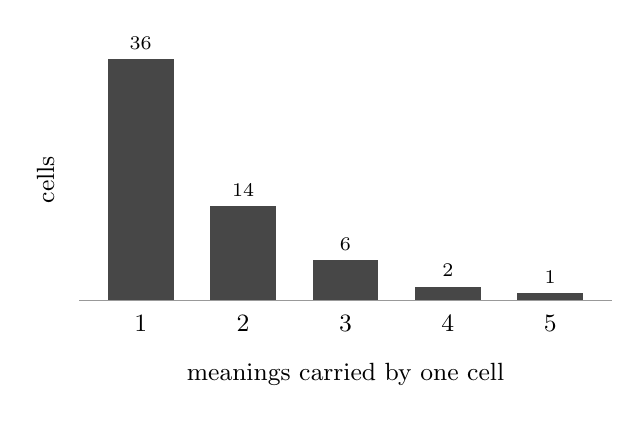
\begin{tikzpicture}[x=13mm, y=9mm]
\draw[black!40] (0.4,0) -- (5.6,0);
\draw[fill=black!72, draw=none] (1-0.32,0) rectangle (1+0.32,3.400);
\node[font=\scriptsize, anchor=south] at (1,3.400) {36};
\draw[fill=black!72, draw=none] (2-0.32,0) rectangle (2+0.32,1.322);
\node[font=\scriptsize, anchor=south] at (2,1.322) {14};
\draw[fill=black!72, draw=none] (3-0.32,0) rectangle (3+0.32,0.567);
\node[font=\scriptsize, anchor=south] at (3,0.567) {6};
\draw[fill=black!72, draw=none] (4-0.32,0) rectangle (4+0.32,0.189);
\node[font=\scriptsize, anchor=south] at (4,0.189) {2};
\draw[fill=black!72, draw=none] (5-0.32,0) rectangle (5+0.32,0.094);
\node[font=\scriptsize, anchor=south] at (5,0.094) {1};
\foreach \k in {1,...,5}{\node[font=\small, anchor=north] at (\k,-0.08) {\k};}
\node[font=\small, anchor=north] at (3.0,-0.75) {meanings carried by one cell};
\node[font=\small, rotate=90, anchor=south] at (0.25,1.7) {cells};
\end{tikzpicture}}

\newcommand{\WorkedSindhi}{\sd{هن} \sd{۾} 8 + 9 = 17 \sd{آهي؟}}
\newcommand{\WorkedBack}{\sd{هن} \sd{۾} 8 + 9 =17 \sd{آهي؟}}
\newcommand{\WorkedGroups}{%
\begin{tabular}{ccccccc}
\bcell{1,2,5} \bcell{1,3,4,5} & \bcell{1,3,4} \bcell{2,4} \bcell{1,3,4,5} & \bcell{3,4,5,6} \bcell{1,2,5} & \bcell{5,6} \bcell{2,3,5} & \bcell{3,4,5,6} \bcell{2,4} & \bcell{5,6} \bcell{2,3,5,6} \bcell{3,4,5,6} \bcell{1} \bcell{1,2,4,5} & \bcell{3,4,5} \bcell{1,2,5} \bcell{2,4} \bcell{2,3,6} \\[3pt]
{\scriptsize\ttfamily 125\,1345} & {\scriptsize\ttfamily 134\,24\,1345} & {\scriptsize\ttfamily 3456\,125} & {\scriptsize\ttfamily 56\,235} & {\scriptsize\ttfamily 3456\,24} & {\scriptsize\ttfamily 56\,2356\,3456\,1\,1245} & {\scriptsize\ttfamily 345\,125\,24\,236} \\
\end{tabular}}
\newcommand{\NWorkedGroups}{7}


\usepackage{bidi}                      % must be loaded last
\newcommand{\sd}[1]{{\sdfont\RL{#1}}}
% Inside maths \RL is unavailable, and every Sindhi mark used in a formula
% here is a single glyph, which needs no reordering.
\newcommand{\sdm}[1]{\text{\sdfont #1}}

\title{\bfseries Standard Sindhi Braille in software:\\
implementing and verifying a ratified national braille code}

\author{%
  Safeer Ali Mirani\thanks{Software implementation, verification suite,
  documentation and evaluation design.} \and
  Riaz Hussain Memon\thanks{Member of the committee that authored the code;
  blind teacher; President, Pakistan Association of the Blind (Sindh).
  Contributed the source material, the rulings recorded in
  \S\ref{sec:reading}, and the reading by touch.}%
}
\date{}

\begin{document}
\maketitle

\begin{abstract}
\noindent
Standard Sindhi Braille was ratified on 7 November 2016 by a committee of the
Sindhi Language Authority and has been taught in schools and read by touch in
Sindh since. Until the work reported here it had no software implementation:
no program could produce a line of it. \texttt{liblouis}, the open braille
translation library, does ship a table under the language code \texttt{sd}, but
it is an unverified stub that includes a Devanagari table written for Sindhi as
it is written in India, and it cannot render a letter of the Perso-Arabic script
Pakistan uses. We report the first digital implementation of the ratified
code. The central difficulty is
structural rather than notational. Sindhi is written with \NLetters{} letters
and the code must express \NMeanings{} distinct marks as single cells, against
the 63 forms a six-dot cell can take, so forward translation is a function and
its inverse is not: \NShared{} cells carry more than one reading and
\NThreeWay{} carry three or more. We give the resolution procedure, which is
positional in all but one case and lexical in that one, and we report its
measured cost. The implementation comprises a reference translator, a pair of
\texttt{liblouis} tables that compile and pass a 99-case suite, and a second,
independent engine written to the same specification so that disagreements
between implementations become observable. Verification runs at five levels, the
last of which is a reading by touch: on 15 August 2026 the second author read an
embossed page produced by this software, without prior sight of the text,
complete and without error. We report one rule the verification design could not see, because it compared
cells and not the spaces between them, and what we changed so that it can. We
also report four points on which the printed standard contradicts itself, which
are matters for the Authority rather than for us.
\end{abstract}

\section{Introduction}

A braille code is a decision, taken by people, about which of the sixty-three
arrangements of six raised dots stands for which mark of a writing system. Once
taken, the decision has to be implemented in software, or it reaches few
readers: a code no program knows cannot be produced by a screen reader, cannot
be embossed from an electronic document, and cannot turn an arbitrary text into
something a blind reader can hold.

Sindhi is the third most widely reported mother tongue in Pakistan. The 2023
census recorded 14.3\% of a population of 247{,}541{,}947, or roughly 35
million speakers \cite{pbs2023}. It is written in a Perso-Arabic script of
\NLetters{} letters. Its braille code was settled in 2016 and is in daily use in
schools in Sindh. It had no implementation.

The absence is worth stating precisely, because at first glance it looks as
though it has been filled. \texttt{liblouis} 3.29.0 ships \texttt{sd.tbl},
indexed as \emph{Sindhi braille}. The file carries the maintainers' own note
that its metadata ``hasn't been verified by the table author yet'', and its
substance is a single \texttt{include} of \texttt{si-in-g1.utb}, a 2014 table
from the Braille Council of India whose header describes it as Sindhi Grade 1
and which in turn includes \texttt{devanagari.cti}. It therefore serves Sindhi
as written in India, in Devanagari, on Bharati Braille lines. It contains
nothing that can render the Perso-Arabic script, and it predates the 2016 code
by two years. A user selecting ``Sindhi'' in a screen reader on a Pakistani
Sindhi document gets a table for a different script.

This paper reports that implementation and, at greater length, how it was
checked. We take the checking to be the more transferable contribution. A
braille code for a language in this position is an unusual object to implement:
it is defined by a printed document and by a small number of people who read it
by touch, and neither a held-out test set nor a large corpus can substitute for
either. What we describe is a way of arranging evidence so that each level
catches a class of error the others cannot.

\subsection{Contributions}

\begin{enumerate}
\item The first software implementation of Standard Sindhi Braille: a reference
      translator in both directions, \texttt{liblouis} tables for Grade 1 and
      Grade 2, and a second independent engine.
\item A formal statement of the shared-cell problem for this code, with all
      counts derived from the implemented tables rather than asserted, and a
      resolution procedure whose single irreducible case we characterise
      exactly.
\item A five-level verification design and its results, including a reading by
      touch by a blind reader who is also an author of the code.
\item Four self-contradictions in the printed standard, reported rather than
      silently resolved.
\end{enumerate}

\section{Related work}

\paragraph{Braille translation infrastructure.}
\texttt{liblouis} \cite{egli2009,liblouis} is an open braille translation
and back-translation library. Its design is table-driven: a language is
supported by contributing a table, which then becomes available to every
application that links the library. This makes the table, rather than any single
application, the artefact that determines whether a language is served, and it
is why we treat producing a correct table as a primary contribution rather than
a packaging step.

It also means that a language can appear supported when it is not. The
\texttt{sd.tbl} case described in \S1 is an instance: an index entry, a
display name, and an \texttt{include} of a table for a different script. We
mention it not as a criticism of the maintainers, whose comments in the file say
plainly that the entry is unverified, but because it changes what an
implementation for a language in this position has to establish. It is not
enough to show that no table exists; one has to show what the existing entry
actually does.

\paragraph{Documentation of braille codes.}
\emph{World Braille Usage} \cite{wbu2013} is the standard survey of braille
codes by country and language. Its third edition lists the braille languages of
Pakistan as Urdu and English (p.\ 103). Standard Sindhi Braille was ratified
three years after that edition appeared, so its absence is chronological rather
than a judgement, but it does describe the situation this work addresses: the
code is not represented in the reference literature that implementers consult.

\paragraph{Perso-Arabic braille in software.}
Work on the neighbouring codes is closest to ours. Akram et al.\
\cite{akram2020} report an Urdu braille editor, and note the same absence of
support for a Perso-Arabic braille code in existing tools that motivates this
paper. Iqbal et al.\ \cite{iqbal2017} address the other half of the problem, the
sighted parent or teacher who does not read braille, with an interactive Urdu
braille learning system. Sindhi differs from Urdu in ways that matter for a
translator rather than only for a font: it has letters Urdu does not, notably
\sd{ڪ}, and \S\ref{sec:neighbours} shows that this is precisely where the two
codes must diverge.

\paragraph{Braille codes as living standards.}
The Rules of Unified English Braille \cite{iceb2024} illustrate that a braille
code is revised, and that its rules are stated at a level of detail an
implementation must respect: \S11.2 of that rulebook treats the spacing of
operation signs and of comparison signs as separate questions. That distinction
is directly relevant to one of the questions still open in the Sindhi code
(\S\ref{sec:limitations}).

\paragraph{Sindhi in the other tradition.}
Sindhi is written in India in Devanagari as well as in the Perso-Arabic script,
and Indian braille for Devanagari follows the Bharati scheme. The table
\texttt{si-in-g1.utb} discussed above belongs to that tradition. The two
codes are not variants of one another: they share neither the script, nor the
alphabet, nor the cell assignments, and a reader of one cannot read the other.
This paper concerns only the Perso-Arabic code ratified in Pakistan.

\paragraph{What is not addressed here.}
A separate literature treats the recovery of text from images of embossed
pages. That is a different problem with different inputs, and nothing in this
work depends on it. Our input is electronic text and our output is an
electronic braille file.

\section{The code and its provenance}

Standard Sindhi Braille was given final form on 7 November 2016 under the
patronage of the Sindhi Language Authority, an autonomous institution of the
Government of Sindh. A committee of six agreed it unanimously: Prof.\ Dr Abdul
Ghafoor Memon (Chairman), Shahid Ahmed Memon (Convener), Riaz Hussain Memon,
Prof.\ Mehrab Ali Lakho, Dr Saira Saleem Khan and Shamsuddin Shaikh, certified
by Haroon Inayat Abbasi, Secretary. The Government of Sindh prints school
textbooks in the code through the DEPD Braille Press, Karachi.

The code is documented in the Authority's printed guide \cite{guide2016} and in
the second author's Grade 1 and Grade 2 teaching books \cite{memon-g2}.
Everything implemented here derives from those documents. We have altered
nothing: where the printed material is ambiguous or inconsistent we report it in
\S\ref{sec:contradictions} rather than choosing silently.

\section{The structure of the problem}
\label{sec:problem}

\subsection{The cell}

\begin{figure}[t]
\centering
\begin{LTR}
\begin{tikzpicture}[
    lbl/.style={font=\small, align=center, text width=38mm, anchor=north}]
  % the six positions, numbered
  \begin{scope}[x=7mm, y=7mm]
    \foreach \d/\x/\y in {1/0/2, 2/0/1, 3/0/0, 4/1/2, 5/1/1, 6/1/0} {
      \draw[black!35] (\x,\y) circle (0.30);
      \node[font=\small] at (\x,\y) {\d};
    }
  \end{scope}
  \node[lbl] at (0.35,-0.75) {the six positions\\and their numbers};
  % one cell
  \node at (5.4,0.7) {\Large\bcell{1,3}};
  \node[lbl] at (5.4,-0.75) {dots 1-3\\the letter \sd{ڪ}};
  % two cells
  \node at (10.4,0.7) {\Large\bcell{1,3}\,\Large\bcell{2,3,6}};
  \node[lbl] at (10.4,-0.75) {dots 1-3 then 2-3-6\\the letter \sd{ک}};
\end{tikzpicture}
\end{LTR}
\caption{The braille cell and its dot numbering, and the two-cell letter
discussed in \S\ref{sec:neighbours}. Throughout this paper a raised dot is
drawn solid and an unraised position faint, following the convention of the
committee's printed guide.}
\label{fig:cell}
\end{figure}

A six-dot cell has $2^{6}-1 = 63$ non-empty forms (Figure~\ref{fig:cell}).
Counting only those marks the code writes as a single cell standing alone, our
implementation assigns \NMeanings{} distinct meanings across \NCellsUsed{} of
those 63 forms. Including marks written as two cells, all 63 are used.

\subsection{More to say than there are cells}

Let $\Sigma$ be the set of marks the code must express and $\mathcal{B}$ the set
of cells. Forward translation is a map
\[
T:\Sigma^{*}\longrightarrow\mathcal{B}^{*},
\]
total and well defined. It is not injective. Since $|\Sigma| > |\mathcal{B}|$,
collisions are forced, and the code has them: \NShared{} cells carry more than
one reading and \NThreeWay{} carry three or more
(Figure~\ref{fig:readings}). The two most heavily loaded are
\[
R(\text{dot }2)=\{\,\text{zabar},\ \sdm{،},\ \text{decimal point},\
\text{lower }1,\ \text{pen-name mark}\,\}
\]
\[
R(\text{dots }2\text{-}3\text{-}6)=\{\,\sdm{ھ},\ \sdm{؟},\ \text{lower }8,\
\text{open quote}\,\}.
\]

Back-translation is therefore not the application of an inverse. Given $\beta
\in \mathcal{B}^{*}$ it is the problem of finding some $w$ with $T(w)=\beta$ and
choosing among the candidates.

\begin{figure}[t]
\centering
\begin{LTR}
\ReadingsHistogram
\end{LTR}
\caption{How many meanings each cell carries, over the \NCellsUsed{} cells the
code assigns as single cells. The \NThreeWay{} cells in the right-hand three
columns are where back-translation needs more than a table.}
\label{fig:readings}
\end{figure}

\subsection{Position resolves almost everything}

The code is constructed so that most collisions are resolved by where a cell
sits, and these can be stated as predicates on the index. The clearest case is
dots 3-4-5-6:
\[
c = 3456 \;\longmapsto\;
\begin{cases}
\text{number sign} & \text{if } i = 0\\
\sdm{ڻ} & \text{otherwise.}
\end{cases}
\]
This is sound only if no ordinary Sindhi word begins with \sd{ڻ}. We measured
the claim rather than assuming it. Over 23{,}432 word tokens drawn from the
committee's own publications, \sd{ڻ} occurs 604 times inside or at the end of a
word and 18 times at the start of a token. Seventeen of those 18 are the bare
letter standing alone, which is what a book about the alphabet contains rather
than what running prose does. The eighteenth is the aspirate \sd{ڻھ}.

That exception is already accounted for elsewhere in our measurements:
\sd{ڻھ} is one of the four spellings the round-trip check reports as not
surviving (\S\ref{sec:suite}), because its two cells are also the fraction
$1/8$. The rule is sound for prose, and its single failure is counted in the
fidelity figure rather than excluded from it.

Dots 2-5-6, 2-3-5 and 2 resolve on word-final position; dots 2-5 resolves by
look-ahead, since a ratio is followed by a fresh number sign and a fraction
denominator is not.

\subsection{One case position cannot resolve}
\label{sec:irreducible}

At the end of a word, dots 2-3-6 is either the letter \sd{ھ} or the question
mark \sd{؟}, and the guide places the question mark in exactly the position a
final \sd{ھ} occupies. No positional predicate separates them. Here the software
makes a decision rather than applying a rule: given the stem $s$ and a lexicon
$W$,
\[
\hat{x} =
\begin{cases}
\sdm{ھ} & \text{if } s\cdot\sdm{ھ} \in W\\
\sdm{؟} & \text{else if } s \in W\\
\sdm{ھ} & \text{otherwise.}
\end{cases}
\]
A human reader resolves this from the sense of the sentence. Lacking that, the
software uses the lexicon, and where the lexicon is silent falls back on the
prior, final \sd{ھ} being far the commoner. We report this as a limitation, not
as a solved case.

\subsection{Rules with scope beyond the character}

Cell-by-cell substitution handles much of Sindhi and then fails, because several
rules are not local. A repeated word is written once and marked. A date is a
construction rather than a sequence of digits with separators. A fraction places
the numerator in upper digits and the denominator in lower ones, which are
different cells for the same digits, so the translator must know which half of
the fraction it is in. Each requires state across a span longer than one
character, which is why the implementation is a transducer rather than a table.

\section{The alphabet}

\AlphabetTable

\section{The cells that carry more than one reading}

Table~\ref{tab:ambiguity} is generated from the implemented tables, so it cannot
drift from them.

\AmbiguityTable

\section{Implementation}

\begin{figure}[t]
\centering
\begin{LTR}
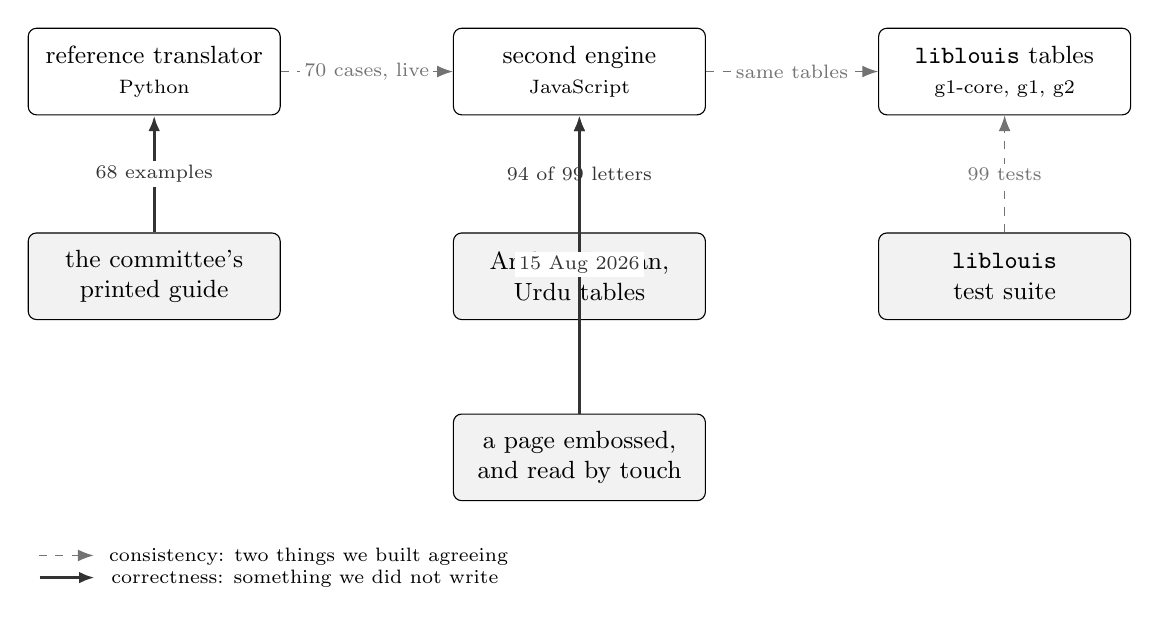
\begin{tikzpicture}[
   font=\small,
   impl/.style={draw, rounded corners=3pt, align=center, inner sep=5pt,
                minimum height=11mm, minimum width=32mm, fill=white},
   ev/.style={draw, rounded corners=3pt, align=center, inner sep=5pt,
              minimum height=11mm, minimum width=32mm, fill=black!5},
   cons/.style={-{Latex[length=2mm]}, black!55, dashed},
   corr/.style={-{Latex[length=2mm]}, black!80, very thick},
   lab/.style={font=\scriptsize, inner sep=1.5pt, fill=white}]

  % the three implementations, in a row
  \node[impl] (py)  at (0,0)      {reference translator\\{\scriptsize Python}};
  \node[impl] (js)  at (5.4,0)    {second engine\\{\scriptsize JavaScript}};
  \node[impl] (lou) at (10.8,0)   {\texttt{liblouis} tables\\{\scriptsize g1-core, g1, g2}};

  % the evidence, below
  \node[ev] (book)  at (0,-2.6)   {the committee's\\printed guide};
  \node[ev] (nb)    at (5.4,-2.6) {Arabic, Persian,\\Urdu tables};
  \node[ev] (suite) at (10.8,-2.6){\texttt{liblouis}\\test suite};
  \node[ev] (touch) at (5.4,-4.9) {a page embossed,\\and read by touch};

  \draw[cons] (py) -- node[lab]{70 cases, live} (js);
  \draw[cons] (js) -- node[lab]{same tables} (lou);
  \draw[corr] (book) -- node[lab]{68 examples} (py);
  \draw[corr] (nb)   -- node[lab]{94 of 99 letters} (js);
  \draw[cons] (suite)-- node[lab]{99 tests} (lou);
  \draw[corr] (touch) -- node[lab]{15 Aug 2026} (js);

  \node[align=left, anchor=west, font=\scriptsize] at (-1.6,-6.3)
   {\tikz{\draw[cons](0,0)--(0.7,0);}~~consistency: two things we built agreeing\\
    \tikz{\draw[corr](0,0)--(0.7,0);}~~correctness: something we did not write};
\end{tikzpicture}
\end{LTR}
\caption{The three implementations and what checks what. The arrows from the
printed guide are the only ones that can establish correctness rather than
consistency; the arrow to \emph{read by touch} is the only one that leaves the
software entirely.}
\label{fig:arch}
\end{figure}

Three implementations exist, deliberately (Figure~\ref{fig:arch}).

\paragraph{The reference translator.} Python, both directions, Grade 1 and
Grade 2. It is the definition, in the sense that the other two are checked
against it.

\paragraph{The \texttt{liblouis} tables.} A shared core
(\texttt{sd-pk-g1-core.uti}) with a Grade 1 table (\texttt{sd-pk-g1.utb}) and a
Grade 2 table (\texttt{sd-pk-g2.ctb}). Both compile without error under
\texttt{liblouis} 3.29.0, and the accompanying test suite passes 99 tests with
0 failures. This is the artefact that lets a screen reader or an embosser use
the code without knowing anything about this project.

\paragraph{The second engine.} An independent implementation in JavaScript, so
that a translator runs with nothing installed and no text leaving the machine.
Its role in the verification design is that it can disagree with the reference
implementation, and it has: the disagreements it exposed are described in
\S\ref{sec:suite}.

\begin{figure}[t]
\centering
\begin{LTR}
\WorkedGroups
\end{LTR}
\smallskip

{\small reads back as \WorkedBack{}}
\caption{One sentence carried through: \WorkedSindhi{}. Four rules fire at once.
The second group is the sign \sd{۾}, which has no cell of its own and is written
out as the word it stands for. The third and fifth carry the number sign. The
sixth is the equals sign closed up to the 17, which is how the guide sets every
one of its worked sums (\S\ref{sec:arith}). The last cell of the last group is
dots 2-3-6, which at the end of a word is either \sd{ھ} or \sd{؟} and is
settled here only by the lexicon (\S\ref{sec:irreducible}).}
\label{fig:worked}
\end{figure}

\subsection{Grade 2}

Grade 2 is contracted braille, and it is what Sindhi braille books use. The
implementation covers 237 contractions in six prefix series plus a set of
abbreviations, and six \sd{ڳانڊڙا} groups written inside a word. The six prefix
series correspond to Louis Braille's seventh line, $\{4,5,6,45,46,56,456\}$, of
which six of the seven head a series here.

The source material states the contractions but nowhere states \emph{when} a
contraction may be used. Placement rules are therefore not implemented, and we
record this as an omission in the source rather than in our reading of it.

\section{Verification}

\subsection{The design}

Five levels, each catching what the others cannot.

\begin{enumerate}
\item \textbf{The software against itself.} Round-trip fidelity, internal
      consistency, rebuild determinism.
\item \textbf{The software against the printed standard.} Every worked example
      the guide prints, reproduced cell for cell.
\item \textbf{The software against codes written by other people.} The Arabic,
      Persian and Urdu \texttt{liblouis} tables, none of which have authority
      over Sindhi but all of which share most of its letters.
\item \textbf{A sighted check by an author of the code}, reading dot numbers.
\item \textbf{A reading by touch, from embossed paper, without prior sight of
      the text.}
\end{enumerate}

Levels 1 to 3 are automated and run in minutes. Level 5 is the only one whose
evidence comes from outside the software, and it consumes a reader's time, which
is why the cheaper levels exist: a fault the suite can catch should not be
spending a person's afternoon.

\subsection{What the suite reports}
\label{sec:suite}

\begin{table}[htbp]
\centering
\VerificationTable
\caption{The verification suite, as run. \texttt{skip} is not \texttt{pass}:
where \texttt{liblouis} is not installed the suite says so and reports it
separately.}
\label{tab:suite}
\end{table}

\NChecksPassed{} of \NChecks{} checks pass on a machine without
\texttt{liblouis} installed; on one with it, all \NChecks{} pass. Two figures
deserve comment.

\paragraph{Round-trip fidelity.} For a corpus of word types $w$ with
frequencies $f(w)$,
\[
\rho = \frac{\sum_{w} f(w)\,[\,T^{-1}(T(w)) = w\,]}{\sum_{w} f(w)}.
\]
Measured over 23{,}432 tokens (2{,}702 types) drawn from the committee's own
publications, $\rho = 0.9994$. The residue is four spellings, of which the
principal one is an abbreviation whose reading requires sentence context.

\paragraph{Grade 2.} 238 of 243 contractions survive both directions. The five
that do not are cells the source assigns to two different words. They are a
property of the code rather than a defect of the implementation.

\paragraph{What the second engine caught.} Requiring two implementations to
agree is only useful if disagreement is possible and is acted on. Two of the
faults reported in \S\ref{sec:reading} were found this way: the two engines
were carrying different word lists, and the download width defaulted
differently in the two. Both were invisible to any check that consulted a single
implementation.

\subsection{Corroboration from unrelated codes}
\label{sec:neighbours}

Sindhi shares most of its letters with Arabic, Persian and Urdu, whose
\texttt{liblouis} tables were written by other people, for other languages,
before this project. Where three unrelated codes independently place a letter in
the cell we place it, a transcription error on our part is unlikely.

Of 99 shared letters, 94 agree. Each of the five disagreements has a reason
visible in the alphabet. Arabic assigns \sd{پ}, \sd{چ} and \sd{گ} the cells
Sindhi has already spent on \sd{ب}, \sd{ج} and \sd{ڪ}; Arabic has no \sd{ڪ} and
treats the other three as borrowings, whereas Sindhi treats them as native.
Persian and Urdu write \sd{ک} as dots 1-3, which in Sindhi is \sd{ڪ}, a letter
neither language has; Sindhi cannot reuse the cell and marks its second $k$ by
adding \sd{ھ}, giving two cells (Figure~\ref{fig:cell}).

This last case is where our implementation was once wrong. The printed guide's
dots appeared on four pages to show a single cell. The second author's chart and
his printed Grade 2 book both give two. We followed the books; Persian and Urdu
braille, written by neither of us, corroborate them; and the second author
confirmed it directly on 15 August 2026. We conclude that the dots printed on
those four pages are a typesetting fault rather than a rule.

\subsection{A spacing rule the checks could not see}
\label{sec:arith}

The suite compared cells. It did not compare where the spaces fall, and the
distinction cost us a rule.

The guide prints five worked sums. Reading them for their typography rather
than their cells: every one of its six equals signs is set closed up to the
number that follows, with a space before it, and never with a space after. Our
software wrote a space on both sides. The check that should have caught this
recorded the expected grouping from our own output rather than from the page,
and since the file writer puts exactly one space between groups, the grouping
\emph{is} the spacing. The expectation and the implementation agreed with each
other and neither agreed with the book.

The second author had told us the rule on 15 August 2026, in his own words and
before any of this was checked: a sign takes a space before it and none after.
We recorded it as an open question because we believed the guide contradicted
him. The guide does not contradict him; we had misread it.

Both engines now close a comparison sign up to the number after it, and four of
the five printed sums reproduce exactly. The fifth does not, and we have not
made it: the guide closes \texttt{+} up to the 9 but spaces \texttt{$-$},
\texttt{$\times$} and \texttt{$\div$}, so on operation signs it is one against
three with itself. We follow the three, record the one we fail in the suite
rather than deleting it, and leave the question for the reader who can settle
it.

Two things generalise from this. A check that compares only the units of a
notation cannot see rules about the space between them, and a stored
expectation regenerated from the implementation it is meant to check is not a
check at all. The second was true elsewhere in this project too: the
cross-check between the two engines compared the browser against a file of
answers the Python had produced on some earlier date, so the two could drift
without the check noticing, and they had. It now computes the reference answers
on every run.

\subsection{The reading}
\label{sec:reading}

On 15 August 2026 the second author was given an embossed page produced by this
software: a passage of Sindhi news prose he had not previously seen, six
sentences, containing proper nouns, digits, foreign names and a comma-heavy
structure. He read it through by touch, without correction and without omission.

This is the only check in the project that originates outside it. Every other is
one implementation checking another, or software checking a book.

It establishes that the code as this software writes it is readable as Sindhi
across ordinary running prose. It does not establish that every rule is correct.
It was one reader and one page, and the passage contained no verse, no
arithmetic and no contractions.

\subsubsection{What the reading found}

Six observations followed. Two were settled at once, two are implemented, two
remain open.

The most consequential was not about the code. Words were being split across
lines on the embossed page. The file had been produced by the browser engine,
whose download defaulted to 40 cells per line, the international braille-paper
width; the page was A4, which fits 28. The embosser received lines longer than
the paper and broke them itself, at positions bearing no relation to word
boundaries. A braille file has to be written at the width of the machine that
will emboss it.

We report this because it is a class of error the verification design as it then
stood could not reach. Every automated check in it operates on cells: which cell
a mark becomes, and whether the cells translate back. The file was correct at
that level and unreadable on paper, because the fault was in page geometry,
which no cell-level check inspects. It also shows the cost of a default that
differs between two implementations of the same specification: the round-trip
checks compared cells and never compared page width, so the divergence survived
every level below the fifth.

The second author also ruled on a question software cannot decide. Sindhi
\sd{ک} and Urdu \sd{ک} are one Unicode character (U+06A9), worth two cells in
Sindhi and one in Urdu, and nothing in a text records which language a borrowed
word came from. He ruled that no distinction should be made: a Sindhi reader
reads that letter the same way whichever language the word came from. The code
is therefore one script with one value per letter, and the software does not
branch on the language of a word. The alternative would have required inferring
a word's source language in order to select a cell.

\section{Where the printed standard is inconsistent}
\label{sec:contradictions}

Four points, none of which is ours to resolve; all are matters for the Sindhi
Language Authority. We report them because an implementation forces a choice,
and silence would present our choice as the standard's.

\paragraph{Fractions.} Pages 52 and 53 state the rule twice and work nine
examples: numerator in upper digits, denominator in lower digits, no bar, and
the numerator omitted when it is 1. Page 50 instead writes fractions with a
slash cell between two upper digits, and states no rule. We implement the
pp.\ 52--53 rule.

\paragraph{Brackets.} Page 32 gives one set of bracket cells for prose. Page 53
gives a different set for arithmetic, and prints the open square bracket with
the same cell as the open round bracket, which appears to be an error. Prose and
arithmetic may legitimately differ; the apparent error is a separate matter.

\paragraph{One cell, two signs.} Page 31 prints dot 6 for both \sd{شد} and
\sd{بہ زبرون}.

\paragraph{Multiplication and the foreign-word mark.} Both are dots 5-6
followed by dots 2-3-6, on pages 49 and 46 respectively. Our translator
separates them by spacing, since the foreign mark is written attached to its
word and a bare two-cell sequence between two numbers is therefore
multiplication. That rule is ours and not the standard's.

\section{Limitations}
\label{sec:limitations}

\paragraph{One reader.} Every confirmation in this project traces to one person,
who is also an author of the code and of this paper. That is a strength for
authority and a weakness for independence. A second Sindhi braille reader, at a
different school, reading the test sheets without prior sight of them, is the
most valuable evidence we do not have.

\paragraph{No externally produced braille.} Both of our implementations were
written by one person from the same documents, so their agreement establishes
consistency and not correctness. A body of Sindhi braille produced elsewhere, as
an electronic file, would break that circle. We have not obtained one.

\paragraph{Parts of the guide unseen.} We have not seen the guide's own
alphabet table or its final pages and cannot say what they contain.

\paragraph{Grade 2 placement.} Implemented as a set of contractions and not as a
policy for when to contract, because the source states the former and not the
latter.

\paragraph{Not yet upstream.} The \texttt{liblouis} tables reported here
compile and pass their suite, but they have not been submitted to the
\texttt{liblouis} project. Until they are, a user of a stock installation still
reaches \texttt{sd.tbl}. Submission, and the question of whether the existing
\texttt{sd} entry should be renamed to reflect the script it serves, are matters
for the maintainers and for the two communities concerned.

\paragraph{Questions still open.} Three questions are with the second author on
an embossed decision sheet: whether operation signs close up as the guide's
addition example does or take a space as its other three do
(\S\ref{sec:arith}), a distinction the current international code also draws
between operation and comparison signs \cite[\S11.2]{iceb2024}; the position of
the shadda in \sd{الله}; and the treatment of a line-end in verse. Nothing has
been changed in anticipation of the answers.

\section{Availability}

The implementation, the tables, the verification suite and the specification in
English and Sindhi are public under the MIT licence. The braille code itself is
the committee's work and is not licensed by us. Every table and figure of data
in this paper is generated by the script that builds it, from the modules the
software runs on, so the paper cannot report a figure the implementation does
not produce.

\section*{Acknowledgements}

We thank \textbf{Mansoor Ali Kori}, who works with the second author on
composing and has taken part in the meetings throughout, and the members of the
2016 committee, whose code this implements.

\begin{thebibliography}{9}

\bibitem{akram2020}
Iqra Akram, Muhammad Shahab Siddiqui, and Zazilah May.
\newblock Urdu Braille Editor.
\newblock \emph{University of Sindh Journal of Information and Communication
Technology}, 4(3):159--164, 2020.

\bibitem{egli2009}
Christian Egli.
\newblock \emph{Liblouis: a universal solution for Braille transcription
services}.
\newblock 2009.
\newblock \url{https://liblouis.io/presentations/liblouisPaper.pdf}

\bibitem{iceb2024}
International Council on English Braille.
\newblock \emph{The Rules of Unified English Braille}, third edition.
\newblock Edited by Matthew Horspool, 2024.
\newblock \url{https://iceb.org/}

\bibitem{iqbal2017}
Muhammad Zahid Iqbal, Suleman Shahid, and Mustafa Naseem.
\newblock Interactive Urdu Braille learning system for parents of visually
impaired students.
\newblock In \emph{Proceedings of the 19th International ACM SIGACCESS
Conference on Computers and Accessibility (ASSETS '17)}, pages 327--328. ACM,
2017.
\newblock \url{https://doi.org/10.1145/3132525.3134809}

\bibitem{liblouis}
Liblouis: an open-source braille translator and back-translator.
\newblock Software, version 3.29.0.
\newblock \url{https://liblouis.io/}

\bibitem{memon-g2}
Riaz Hussain Memon.
\newblock \emph{Sindhi Braille, Grade II} [\sd{سنڌي بريل درجو} II].
\newblock Teaching manuscript supplied by the author.
\newblock \textsc{[verify the title exactly as printed on the cover before
submission]}

\bibitem{pbs2023}
Pakistan Bureau of Statistics.
\newblock \emph{7th Population and Housing Census, 2023}: population by mother
tongue.
\newblock Government of Pakistan, 2023.
\newblock \textsc{[verify the table number and the exact figure against the
published census tables before submission]}

\bibitem{guide2016}
Sindhi Language Authority.
\newblock \emph{Standard Sindhi Braille Guide}
[\sd{معياري سنڌي بريل رهبر}].
\newblock Hyderabad, Sindh, 2016.
\newblock \textsc{[verify the imprint, place and year against the printed
copy before submission]}

\bibitem{wbu2013}
\emph{World Braille Usage}, third edition.
\newblock Perkins, International Council on English Braille, and National
Library Service for the Blind and Physically Handicapped, Library of Congress,
Washington, D.C., 2013.

\end{thebibliography}

\end{document}
